\documentclass{standalone}

\usepackage{tikz}
\tikzset{
block/.style={rectangle, minimum width=0.75in, minimum height=3em, text centered, align=center, draw=black, fill=blue!30},
arrow/.style={thick,<-,>=stealth},
noarrow/.style={thick}}

\begin{document}
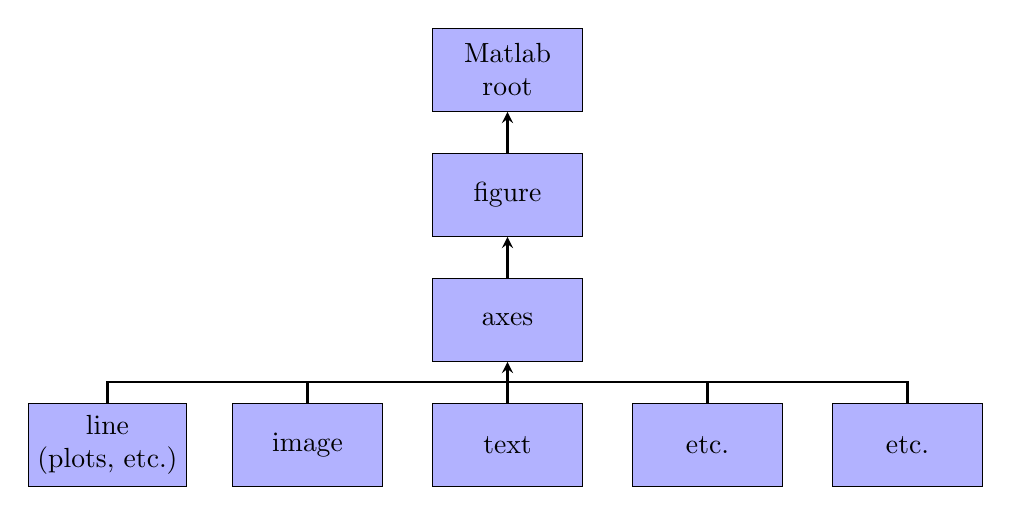
\begin{tikzpicture}
\node (root) [block] {Matlab\\root};
\node (fig1) [block, below of=root, node distance=0.625in] {figure};
\node (ax1) [block, below of=fig1, node distance=0.625in] {axes};
\node (text) [block, below of=ax1, node distance=0.625in] {text};
\coordinate [below of=ax1, node distance=0.3125in] (x); 
\node (image) [block, left of=text, node distance=1in] {image};
\node (line) [block, left of=image, node distance=1in] {line\\(plots, etc.)};
\node (etc1) [block, right of=text, node distance=1in] {etc.};
\node (etc2) [block, right of=etc1, node distance=1in] {etc.};

\draw [arrow] (root) -- (fig1); 
\draw [arrow] (fig1) -- (ax1); 
\draw [arrow] (ax1) -- (text); 
\draw [noarrow] (image) |- (x); 
\draw [noarrow] (line) |- (x); 
\draw [noarrow] (etc1) |- (x); 
\draw [noarrow] (etc2) |- (x); 
\end{tikzpicture}
\end{document}
